\ifbook{

}

\ifslide {

  \begin{frame}{About me...}
    \begin{columns}

    \begin{column}[l]{.3\textwidth}
      \begin{center}
        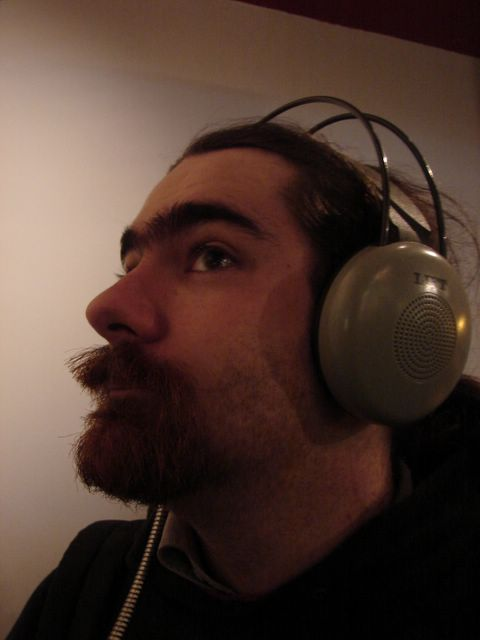
\includegraphics[height=120px]{../img/rpe.jpg}
      \end{center}
    \end{column}

    \begin{column}[r]{.7\textwidth}
      \begin{block}{Romain PELISSE}
        \begin{itemize}
          \item \textbf{Middleware Consultant} at \mylink{http://redhat.com}{Red Hat} (2011)
          \begin{itemize}
            \item Architecte Middleware JBOSS
            \item Red Hat Linux Technician
          \end{itemize}
          \item Committer \mylink{http://pmd.sourceforge.net/}{PMD} and \mylink{http://xradar.sourceforge.net/}{XRadar}
          \item Translation for \mylink{http://www.selenic.com/mercurial/wiki/index.cgi/TranslatingMercurial}{HgBook}
          \item Teach build technologies and OPP at \mylink{http://www.esme.fr/}{ESME Sudria}
        \end{itemize}
      \end{block}
    \end{column}
   \end{columns}
 \end{frame}

 \section{Foreword}

 \begin{frame}
   \begin{block}{Some pratical details}
     \begin{itemize}
       \item I have previous experience in teaching, but to \textbf{technical} people or student
       \begin{itemize}
         \item ... so \textit{stop} me, if I go too fast !
       \end{itemize}
       \item I'm French, but I teach in \textbf{English} because my \textit{Deutsch ist schrecklich}
       \item Session last 3 hours, and are divided into:
       \begin{itemize}
         \item 15 minuten: small MCQ (Multiple choice questionnaire), starting next week
         \item ~1 hour
         \item 30" break
         \item ~1 hour
         \item 15" buffer if we are late or need to go deeper
       \end{itemize}
       \item we are here to \textbf{interact}, not to get your ears used to crappy english spoken by
       French people...
     \end{itemize}
   \end{block}
  \end{frame}

  \begin{frame}
    \begin{block}{Sessions agenda}
       \begin{itemize}
         \item 14h00 bis 17h30 - Freitag 04.05 (1/7 - 3h)
         \item 14h00 bis 17h30 - Freitag 11.05 (2/7 - 3h)
         \item 14h00 bis 17h30 - Freitag 25.05 (3/7 - 3h)
         \item 14h00 bis 17h30 - Freitag 01.06 (4/7 - 3h)
         \item \textbf{14h00 bis 17h30 - Freitag 22.06 (5/7 - 3h)}
         \item 14h00 bis 17h30 - Freitag 29.06 (6/7 - 3h)
         \item 14h00 bis 17h30 - Freitag 13.07 (7/7 - 3h)
      \end{itemize}
    \end{block}

    \begin{block}{Be careful !}
      Those dates can changes (and some will probably) - always checkout on Moodle if a session has
      not been rescheduled
    \end{block}
  \end{frame}

  \begin{frame}
    \begin{block}{Goals}
      \begin{itemize}
        \item Basic understanding of how and why program
        \item Impact in \textbf{your} job
        \item Enhance your communication skills with technical people
      \end{itemize}
    \end{block}

    \begin{block}{Who are you ?}
      \begin{itemize}
        \item Quickly gives us an hint of you are and where you come from...
      \end{itemize}
    \end{block}
  \end{frame}

  % classe outline
  \section{How computer works ?}

  \begin{frame}
    \begin{center}
        What do you know about \textbf{how} a computer work ?
    \end{center}
  \end{frame}

  \begin{frame}
   \begin{center}
     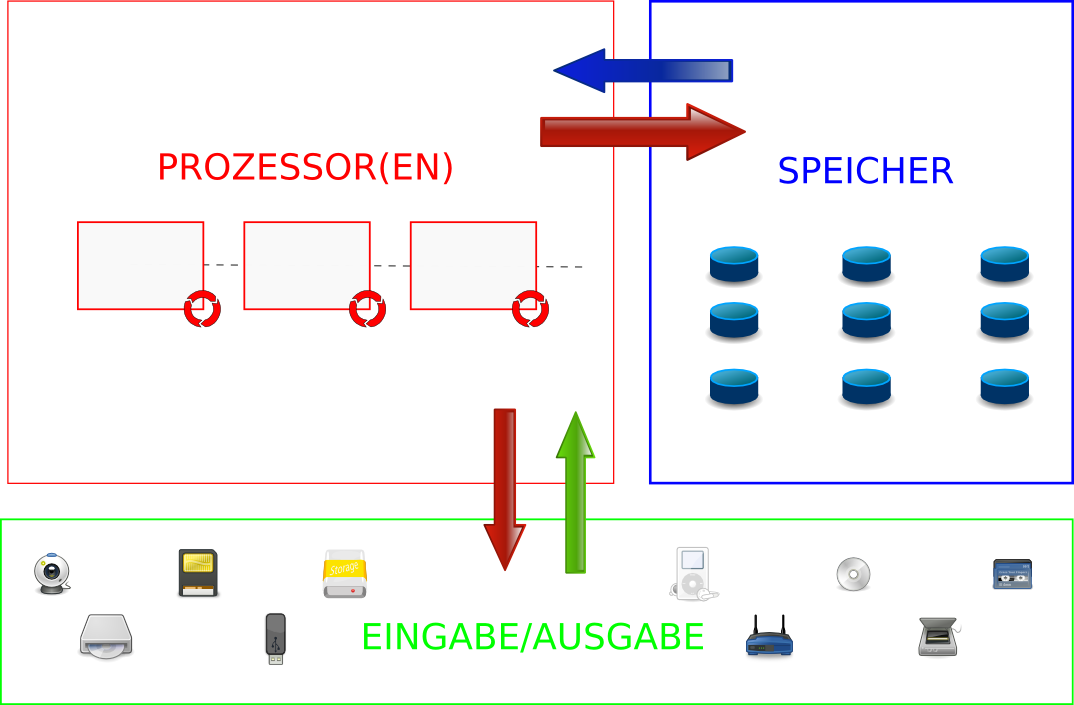
\includegraphics[scale=0.3]{img/cpu-schematics.png}
   \end{center}
  \end{frame}

  \begin{frame}
    \begin{center}
      \begin{itemize}
        \item What is an \textbf{operating system}(OS) ?
        \item Name a few OS names that you know of ?
        \item What does exactly an operating system ? What are its \textbf{responsabilities}?
      \end{itemize}
    \end{center}
  \end{frame}

  \begin{frame}{Role of an Operating System}
    \begin{center}
      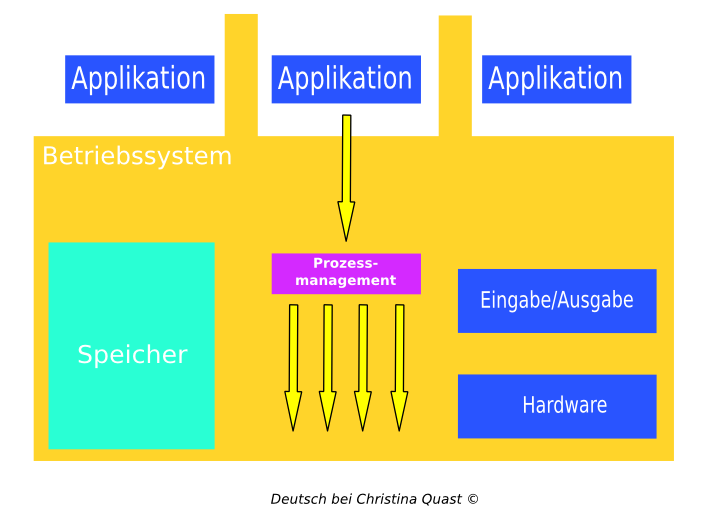
\includegraphics[scale=0.3]{img/operating-system.png}
    \end{center}
  \end{frame}

  \begin{frame}{Speed of I/Os}
    \begin{center}
      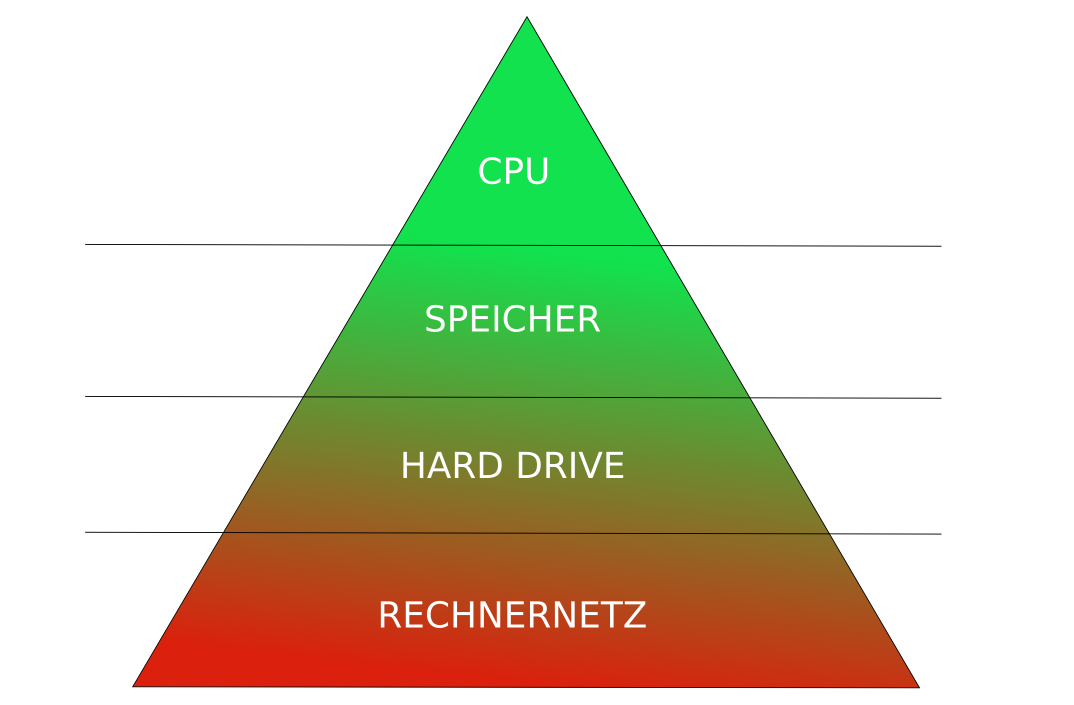
\includegraphics[scale=0.3]{img/pyramid-io.png}
    \end{center}
  \end{frame}

  \section{Short history of IT}

  \begin{frame}{First era of IT: Mainframe and terminals}
    \begin{center}
      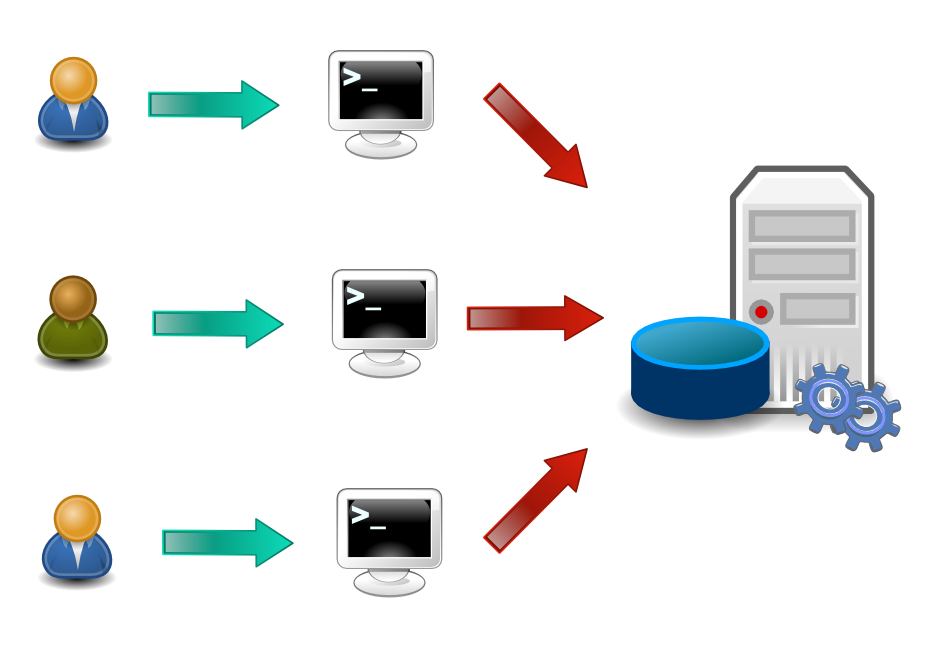
\includegraphics[scale=0.3]{img/mainframe-terminals.png}
    \end{center}
  \end{frame}

  \begin{frame}{Second era of IT: Clients and servers}
    \begin{center}
      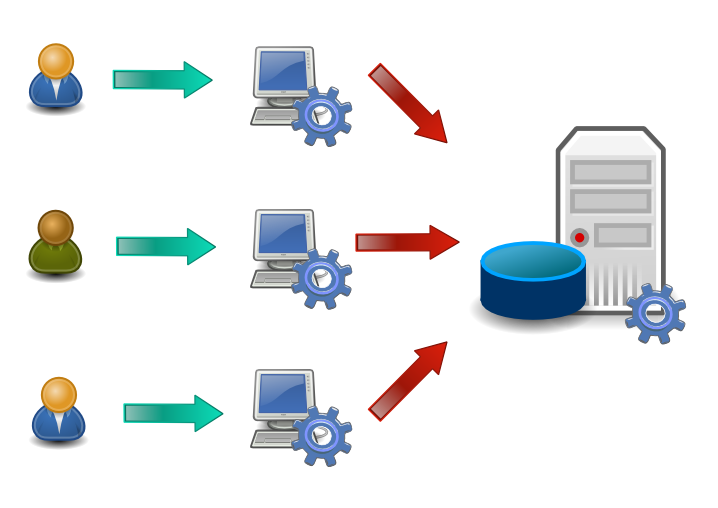
\includegraphics[scale=0.3]{img/fat-clients.png}
    \end{center}
  \end{frame}

  \begin{frame}{Third era of IT: The Internet}
    \begin{center}
      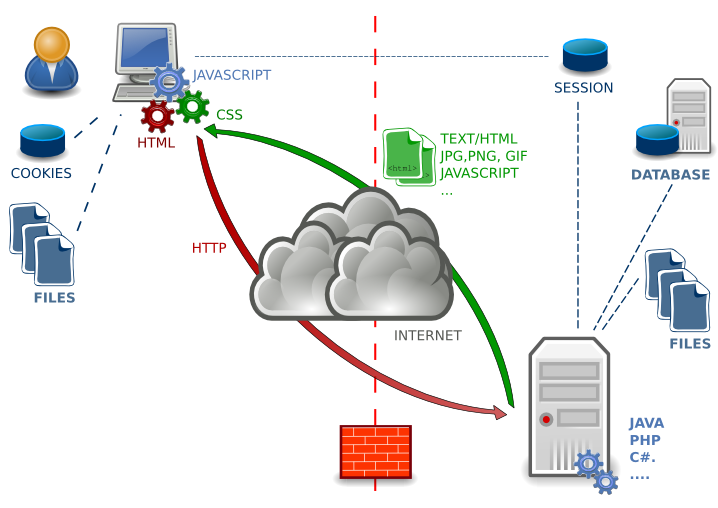
\includegraphics[scale=0.3]{img/internet.png}
    \end{center}
  \end{frame}

  \begin{frame}{Data persistance}
    \begin{center}
      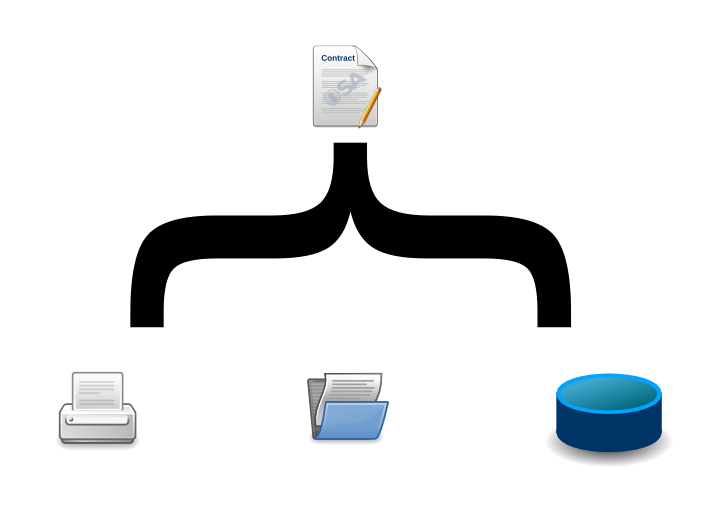
\includegraphics[scale=0.3]{img/persistance.png}
    \end{center}
  \end{frame}

  \section{Java}

  \begin{frame}{Java}
    \begin{block}{What is Java ?}
      \begin{itemize}
        \item \textbf{programming} language
        \begin{itemize}
          \item "look-like" C code
          \item \textbf{Object Programming Oriented}
          \item strongly \textbf{structured}
        \end{itemize}
        \item operating system \textbf{independant}
        \item running within a \textbf{virtual machine}
        \item with automated memory collection
      \end{itemize}
    \end{block}

    \begin{center}
      
\includegraphics[scale=0.2]{img/java-logo.jpg}
    \end{center}
  \end{frame}

  \begin{frame}{Java}
    \begin{block}{Compiling code....}
      \begin{itemize}
        \item What for ? What does it do ? What does it bring ?
        \item Must all languages be compiled ?
        \item If not, what is the point of compiled language ?
      \end{itemize}
    \end{block}
  \end{frame}

  \begin{frame}{Java}
    \begin{block}{The infamous Hello The World program...}
      \begin{itemize}
        \item What is this program ? What does it do ?
        \item Why does programmer always start by writing such a program ?
        \item Let's see how to implement such a program in Java...
      \end{itemize}
    \end{block}
  \end{frame}
}
